\documentclass[11pt,letterpaper]{article}

\usepackage[margin=1in]{geometry}
\usepackage[utf8]{inputenc}
\usepackage[T1]{fontenc}
\usepackage{lmodern}
\usepackage{graphicx}
\usepackage{subcaption}
\usepackage{amsmath,amssymb,amsfonts}
\usepackage{booktabs}
\usepackage{siunitx}
\usepackage{hyperref}
\usepackage{microtype}
\usepackage{float}
\usepackage{caption}

\sisetup{detect-all=true}

\title{A Laminate Parallel Articulated Spine for a Cat-Scale Quadruped Robot}
\author{Jeevan Hebbal Manjunath \and Varun Karthik \and Yeshwanth Reddy Gurreddy}
\date{\today}

\begin{document}
\maketitle

\begin{abstract}
This project presents the design and physical prototyping of a bio-inspired
mechanism intended to serve as the articulated spine of a small quadruped robot
with Jansen mechanisms for its four legs. Taking inspiration from the classical
Sarrus linkage, we develop a planar articulated spine composed of a
three-branch parallel linkage (3R–2R–3R) that connects two rigid 3D-printed
chassis plates and is intended to provide vertical support
while allowing controlled in-plane bending. The spine is realized in a
Smart Composite Microstructures (SCM) format using a five-layer laminate
(rigid--adhesive--flexure--adhesive--rigid). Stiff outer layers form the links,
while the flexure layer creates passive spring-like joints that generate a
restoring torque as the spine bends. The overall morphology is scaled to
roughly match the proportions of a juvenile cat while operating at a much
lower mass of about \SI{250}{g}. We construct both a paper analogue of the
mechanism and a laminate prototype integrated into a quadruped chassis. A planar kinematic model, implemented in Python, represents the
3R–2R–3R parallel spine in the sagittal plane and is used to compute
representative joint torques and joint velocities for expected ground
reaction forces and vertical motions of the front chassis. Using this model, we compute representative joint torques and
joint velocities for expected ground reaction forces and vertical motions of
the front chassis. The results demonstrate that a linkage-based, passively
compliant spine is feasible within the constraints of laminate fabrication and
provides a structured way to tune the directional stiffness of the robot
torso for future integration with Jansen-leg quadruped locomotion.
\end{abstract}

\section{Introduction}
\label{sec:intro}

Bio-inspired legged robots often borrow structural ideas from animals to
improve stability, efficiency, and maneuverability. Many existing quadruped
designs use a rigid torso with compliant legs, or a uniformly flexible
backbone that bends easily in all directions. While these approaches simplify
design and control, they limit the role of the spine to either a passive
connector or a uniformly compliant beam, which can reduce force transmission
and restrict useful body motion during locomotion.

In contrast, animals such as cats and cheetahs rely on spines that are stiff in
some directions and compliant in others, allowing the torso to store and
release energy, extend stride length, and stabilize the body during fast
gaits. Motivated by this idea, this project explores a mechanical articulated
spine for a small quadruped robot driven by Jansen mechanisms at each leg. The design is inspired by the classical Sarrus linkage and realized as a
planar articulated spine composed of a three-branch parallel linkage
(3R–2R–3R) that connects two rigid 3D-printed chassis plates.
The links are made from stiff laminate layers, while the joints are
implemented as thin flexures that behave like passive spring-like hinges due
to the material properties. The goal is to achieve a spine that provides
vertical support, allows controlled in-plane bending, and naturally generates a
restoring torque as it deflects.

This report focuses on the mechanism-level design, scaling, and physical
prototyping of this spine using laminate construction. Dynamic behavior and
full leg--spine coupling are left for future work.

\subsection{Project Rationale and Scope}
\label{subsec:scope}

\textbf{Scope.}  
This project makes the spine the central design element of a small quadruped
platform:
\begin{enumerate}
    \item \textbf{Parallel Articulated Spine.}  
    Design and prototype a Sarrus-inspired planar parallel linkage that
    connects a front and rear chassis, targeting high vertical stiffness with
    controlled in-plane bending between the two bodies.

    \item \textbf{Five-Layer Laminate Implementation.}  
    Fabricate the spine links and joints using a five-layer SCM stack
    (rigid--adhesive--flexure--adhesive--rigid) so that links remain stiff
    while joints behave as compliant, spring-like flexures.

    \item \textbf{Geometric Compatibility with Jansen Legs.}  
    Dimension the spine assuming that each chassis will carry a planar,
    single-degree-of-freedom Jansen leg mechanism that provides a more
    biologically relevant foot trajectory than simple rotary legs, even
    though full leg--spine integration is deferred to later work.
\end{enumerate}

The work in this report is limited to geometric design, basic stiffness
reasoning, and fabrication of spine prototypes using laminate construction with
3D-printed chassis interfaces.

\textbf{Impact.}  
By replacing a rigid or uniformly flexible torso with a parallel articulated
linkage whose joints behave as passive spring-like elements, this project
isolates the spine as a key morphological variable. The prototype provides
initial insight into how a Sarrus-inspired, passively compliant spine can
transmit loads between the front and rear chassis while still permitting
useful bending and self-centering behavior. These results inform future
quadruped designs that must balance support, compliance, and integration with
complex leg mechanisms such as Jansen linkages.

\section{Bio-Inspiration and System Scaling}
\label{sec:bio_inspiration}

\subsection{Biological Basis and Hybrid Concept}

The proposed robot combines two distinct bio-inspired ideas into a single
hybrid morphology. At the \emph{body-plan level}, the platform is scaled to a
small quadruped, roughly corresponding to a juvenile domestic cat with four
primary limbs and a compact trunk. Quadrupeds of this size use their spine to
support body weight while allowing controlled bending in the sagittal plane to
extend stride length and smooth center-of-mass motion during locomotion.

At the \emph{mechanism level}, the internal backbone draws inspiration from
myriapod-style robots that use Sarrus-like linkages to realize segmented,
popup-compatible trunks. Prior centimeter-scale ``micropod'' designs employ
Sarrus mechanisms and laminate flexures to create compliant, vertically
supportive backbones using only revolute joints. In this project we adapt that
idea to a quadruped context: two rigid 3D-printed chassis plates (front and
rear) are connected by a Sarrus-inspired parallel articulated spine,
implemented in a five-layer laminate stack. Stiff outer layers form the links,
while the thin flexure layer creates joints that act as passive torsional
springs and generate a restoring torque as the spine bends.

This results in a hybrid system: externally, the robot resembles a cat-sized
quadruped with four Jansen mechanisms providing leg motion; internally, the
connection between the front and rear bodies behaves like a myriapod-inspired,
Sarrus-based articulated spine.

\subsection{Scale Selection}

The overall geometric and dynamic scale of the robot is chosen to be
proportionally similar to a juvenile cat while keeping the total mass much
lower to match the capabilities of laminate fabrication and small actuators.
Table~\ref{tab:bio_robot_params} summarizes the key parameters used for this
scaling. The robot body length (distance between front and rear chassis) is
set to \SI{0.25}{m}, with an approximate total mass of \SI{0.25}{kg}.

\begin{table}[H]
    \centering
    \caption{Key morphological and locomotion parameters for a juvenile cat and the proposed quadruped robot. Biological values are approximate and used only for scaling.}
    \label{tab:bio_robot_params}
    \begin{tabular}{lccc}
        \toprule
        \textbf{Quantity} & \textbf{Symbol} & \textbf{Juvenile cat} & \textbf{Robot target} \\
        \midrule
        Body mass & $m$ & \SIrange{1.5}{2.0}{kg} & \SI{0.25}{kg} \\
        Body length (shoulder--hip) & $L_{\text{body}}$ & \SIrange{0.25}{0.30}{m} & \SI{0.25}{m} \\
        Typical walking speed & $v$ & \SIrange{0.4}{0.6}{m/s} & \SIrange{0.2}{0.3}{m/s} \\
        Stride length & $L_{\text{stride}}$ & \SIrange{0.30}{0.40}{m} & \SIrange{0.20}{0.25}{m} \\
        Step frequency & $f_{\text{step}}$ & \SIrange{1.5}{2.0}{Hz} & \numrange{1.0}{1.5} \\
        Max foot height (swing) & $h_{\text{foot}}$ & \SIrange{0.03}{0.05}{m} & \SIrange{0.02}{0.03}{m} \\
        Peak vertical GRF per leg & $F_{z,\max}$ & \SIrange{20}{30}{N} & \SIrange{3}{5}{N} (design) \\
        Spine flexion range (sagittal) & $\theta_{\text{spine}}$ & $\approx 10^\circ$ & $\approx 10^\circ$ \\
        \bottomrule
    \end{tabular}
\end{table}

The robot mass is intentionally much lower than that of the biological
counterpart, which reduces expected ground reaction forces and laminate
stresses. With a mass of \SI{0.25}{kg}, the body weight is approximately
\SI{2.45}{N}. Designing for peak vertical ground reaction forces of
\SIrange{3}{5}{N} per leg provides a safety margin for dynamic effects while
remaining compatible with small actuators and laminate flexures.

\subsection{Supporting Literature}

Several prior works inform the specific design and fabrication choices in this project.

\textbf{Bing et al.~\cite{bing}} experimentally demonstrated that lateral spinal flexion in a small legged robot can significantly improve performance and turning behavior. Their results support the focus on spinal stiffness as a key design variable. While their spine is more uniformly compliant, this work extends the idea by investigating a directionally stiff, linkage-based spine with passive spring-like joints.

\textbf{Hoover and Fearing~\cite{hoover_fearing}} established the Smart Composite Microstructures (SCM) process for folded millirobots. This project directly adopts their five-layer laminate methodology---laser-machining rigid layers and laminating them with Kapton flexures---to realize both stiff links and compliant joints in the spine. Their analysis of laminate linkages confirms that mechanisms of similar complexity to the proposed spine (and future Jansen legs) are manufacturable at this scale.

\textbf{Eckert et al.~\cite{eckert}} compared different spine and leg designs for small quadrupeds and showed that spine and leg dynamics are tightly coupled; changes in leg trajectory often require corresponding adjustments in spinal stiffness to maintain efficiency. This motivates designing the spine with explicit consideration of its eventual interaction with Jansen legs, even though only the spine is prototyped here.

\textbf{D\"urr et al.~\cite{duerr}} provided a comprehensive biomimetic foundation for legged locomotion and inter-limb coordination. While their focus is on multi-legged systems, their discussion of stability, duty factor, and phase relationships informs the long-term goal of embedding the articulated spine within a biologically grounded gait framework once the full quadruped (spine + Jansen legs) is assembled.

\paragraph{Novelty.}
Taken together, these works motivate but do not duplicate our approach. Prior robots typically either
use rigid torsos with complex legs, or uniformly compliant spines with simple legs. In contrast, this
project targets a cat-scale quadruped with a linkage-based, directionally stiff spine designed explicitly
for integration with Jansen-style leg mechanisms. To our knowledge, a laminate Sarrus-based spine
configured as the primary torso element of a quadruped has not been previously reported.

\section{Robot Specifications}
\label{sec:specs}

All key physics-based parameters for the proposed quadruped robot are collected
in Table~\ref{tab:robot_specs}. Values are expressed in SI units and are drawn
from biological scaling, material data, or simple calculations as indicated.

\begin{table}[H]
    \centering
    \caption{Specifications table for the proposed quadruped robot.}
    \label{tab:robot_specs}
    \begin{tabular}{lcccl}
        \toprule
        \textbf{Parameter} & \textbf{Symbol} & \textbf{Unit} &
        \textbf{Value / Range} & \textbf{Source} \\
        \midrule
        Total mass & $m$ & \si{kg} & 0.25 & Measured \\
        Body length (shoulder--hip) & $L_{\text{body}}$ & \si{m} &
        0.25 & Geometry, scaled from cat data \\
        Target walking speed & $v$ & \si{m/s} &
        0.2--0.3 & Design goal \\
        Stride length & $L_{\text{stride}}$ & \si{m} &
        0.20--0.25 & Design goal \\
        Step frequency & $f_{\text{step}}$ & \si{Hz} &
        1.0--1.5 & Design goal \\
        Peak vertical GRF per leg & $F_{z,\max}$ & \si{N} &
        3--5 & Scaled from cat GRF data \\
        Body weight & $W = mg$ & \si{N} &
        $\approx 2.45$ & Calculated from mass \\
        Peak COM vertical acceleration & $a_z$ & \si{m/s^2} &
        $\approx 6.2$ & Calculated (this work) \\
        Max spine pitch (front--rear) & $\theta_{\max}$ & \si{rad} &
        $\approx 0.17$ & Design limit \\
        Target spine torsional stiffness & $k_\theta$ & \si{N\,m/rad} &
        $\approx 1.4$ & Calculated (this work) \\
        Laminate link modulus (FR4) & $E_{\text{link}}$ & \si{GPa} &
        15--25 & Datasheet / SCM literature \\
        Flexure modulus (Kapton) & $E_{\text{flex}}$ & \si{GPa} &
        2.5--3.0 & Datasheet / SCM literature \\
        Laminate stack & -- & -- &
        5-layer (rigid--adhesive--flexure--adhesive--rigid) &
        SCM process~\cite{hoover_fearing,aukes_textbook} \\
        \bottomrule
    \end{tabular}
\end{table}

The values in Table~\ref{tab:robot_specs} combine biological scaling and
conservative design choices. The peak ground reaction forces are scaled from
biological values but slightly overestimated to provide a safety margin. The
target walking speed, stride length, and step frequency are reduced relative to
biology to reflect the limitations of small actuators and friction in laminate
joints. The spine pitch limit and corresponding torsional stiffness are design
targets chosen to allow visible bending while maintaining a strong passive
restoring torque from the flexure-based joints.

\section{Physical Mechanism Prototypes}
\label{sec:physical}

\subsection{Paper Mechanism Prototype}

To develop intuition for the articulated spine, we first built a paper
mechanism using slit-and-fold joints. Figure~\ref{fig:fig_prototype} shows the
resulting model in several configurations. The prototype consists of two large
prismatic frames representing the front and rear body segments and a central
spine module built from folded triangular facets. All joints are implemented
as thin paper folds, which act as flexible hinges.

\begin{figure}[H]
  \centering
  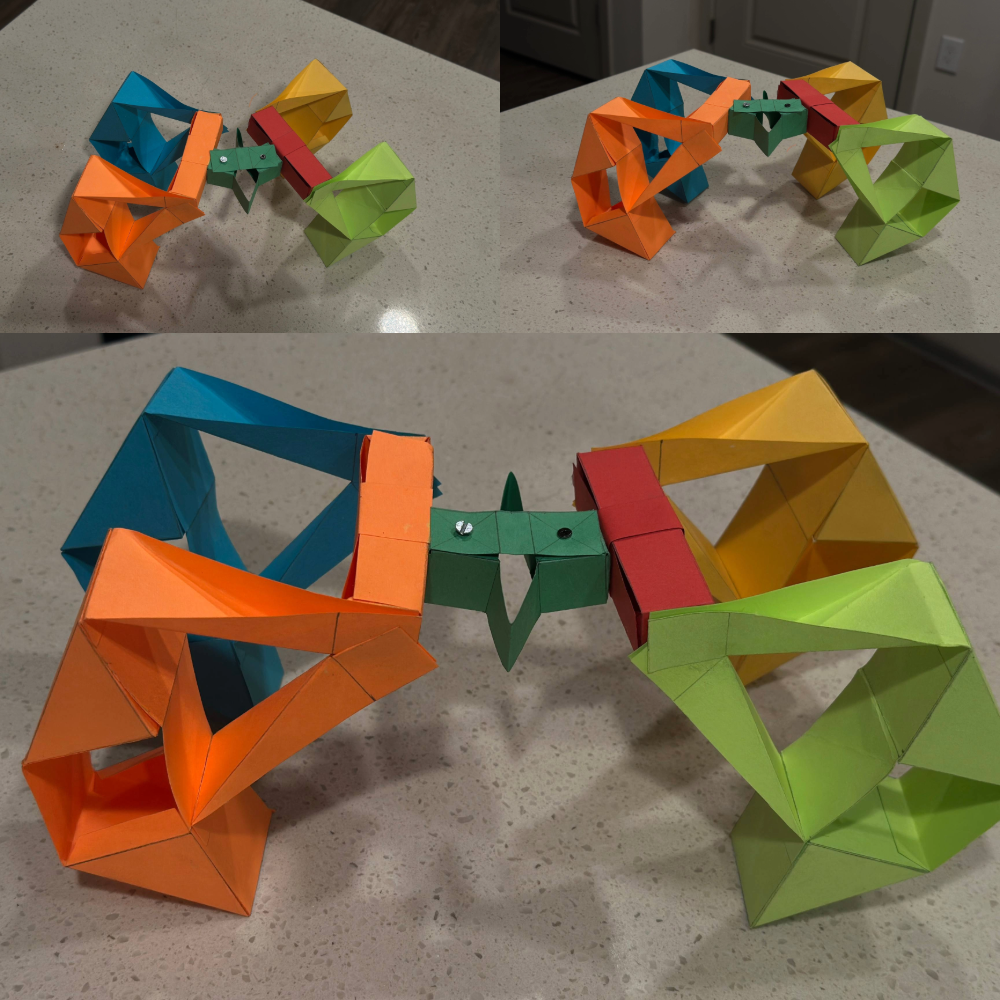
\includegraphics[width=0.9\linewidth]{images/fig_prototype.png} % Image file not found
  \caption{Paper prototype of the articulated spine mechanism in multiple
  configurations. The colored prismatic frames represent the front and rear
  body segments. The central colored elements form a spatial Sarrus-like
  linkage whose folded joints behave as passive hinges. By manually rotating
  the outer frames relative to each other, the spine bends while remaining
  vertically supportive, illustrating the intended behavior of the laminate
  spine in the final robot.}
  \label{fig:fig_prototype}
\end{figure}

This paper analogue validates the qualitative motion of the Sarrus-based
spine and helps identify locations where flexures and rigid links should be
reinforced in the laminate design.

\section{Mechanism Geometry and Kinematic Diagram}
\label{sec:geometry}

The physical spine module is a planar articulated spine composed of a
three-branch parallel linkage (3R–2R–3R) between two rigid platforms
(front and rear chassis). For clarity, we draw a planar
kinematic diagram in the sagittal plane, shown in
Fig.~\ref{fig:images/spine_kinematic_diagram}. The ground link of length $l_0$
connects points $P_6$ and $P_0$, which lie on the rear chassis. Two mirrored
three-link chains connect $P_6$ and $P_0$ to a common point $P_3$, which
represents the front chassis attachment. A central link of length $l_6$
connects $P_6$ to $P_3$ and enforces the parallel relationship between front
and rear platforms.

\begin{figure}[H]
  \centering
  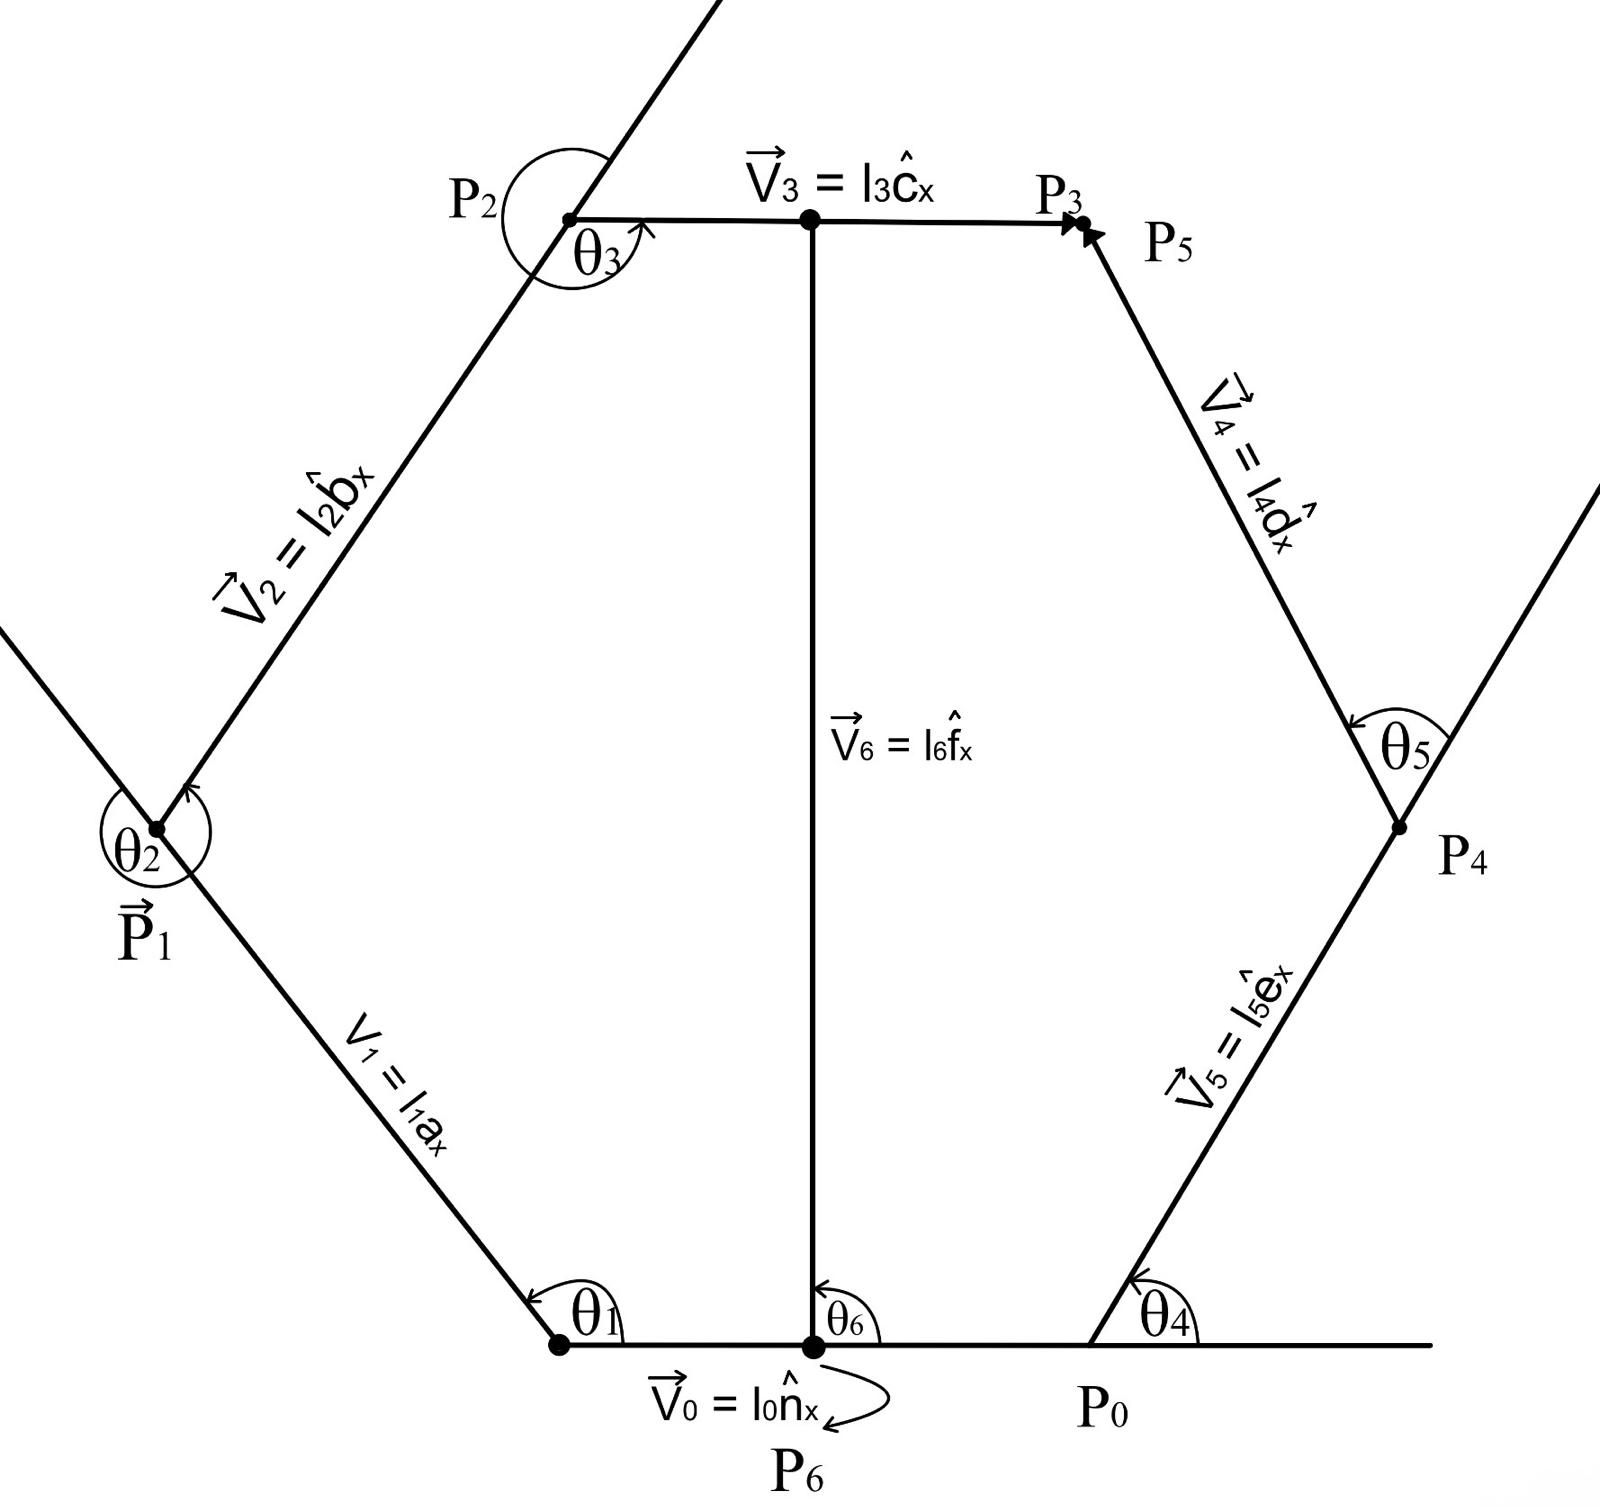
\includegraphics[width=0.85\linewidth]{images/spine_kinematic_diagram.jpeg} % Image file not found
  \caption{Planar kinematic diagram of the articulated spine. The inertial
  frame $\mathcal{N}$ is defined by $\{\hat{n}_x,\hat{n}_y,\hat{n}_z\}$. Rigid
  links are represented by vectors $\vec{V}_i = l_i \hat{(\cdot)}_x$, where
  $l_i$ is the length of link $i$ and the local $\hat{(\cdot)}_x$ axis is
  aligned with that link. Points $P_0$--$P_6$ denote joint locations, and
  joint angles $\theta_1 \dots \theta_6$ are measured relative to the
  $\hat{n}_x$ axis. The full mechanism is a spatial Sarrus-based linkage; here we restrict attention
to motion in the sagittal plane and model the planar 3R–2R–3R parallel spine using
the joint coordinates $\theta_1 \dots \theta_6$ defined above.}
  \label{fig:images/spine_kinematic_diagram}
\end{figure}

\section{Estimated Goal Performance Metrics}
\label{sec:goal_metrics}

The literature provides approximate values for body mass and ground reaction
forces, but it does not directly specify several design metrics important for
the articulated spine. Here we estimate (1) the peak vertical acceleration of
the body during stance and (2) a target torsional stiffness for the spine.

\subsection{Peak Vertical Acceleration}

With total mass $m = \SI{0.25}{kg}$, the robot weight is
\begin{equation}
    W = m g = 0.25 \times 9.81 \approx \SI{2.45}{N}.
\end{equation}
During walking, each leg experiences a peak vertical ground reaction force in
the range of $3$--\SI{5}{N}. We choose a representative value
$F_{z,\max} = \SI{4}{N}$ for a single leg. Assuming that at the instant of
peak force the net vertical force on the body is dominated by the difference
between the ground reaction force and weight, Newton's second law gives
\begin{equation}
    F_{z,\max} - W = m a_z.
\end{equation}
Solving for $a_z$,
\begin{equation}
    a_z = \frac{F_{z,\max} - W}{m}
        \approx \frac{4.0 - 2.45}{0.25}
        \approx \SI{6.2}{m/s^2},
\end{equation}
corresponding to a peak upward acceleration of roughly $0.6g$. This sets a
reasonable target for the vertical dynamics that the articulated spine must
accommodate without excessive deflection.

\subsection{Target Torsional Stiffness of the Spine}

We would like the spine to permit a maximum relative pitch angle of
$\theta_{\max} \approx 10^\circ$ between the front and rear chassis under load
while generating a restoring torque that tends to re-center the body. If we
assume that a disturbance produces an effective moment of
$\tau_{\max} = \SI{0.25}{N\,m}$ about the spine, and model the spine as a
linear torsional spring,
\begin{equation}
    \tau = k_\theta \theta,
\end{equation}
then a target torsional stiffness is
\begin{equation}
    k_\theta = \frac{\tau_{\max}}{\theta_{\max}}
             \approx \frac{0.25}{0.174}
             \approx \SI{1.4}{N\,m/rad}.
\end{equation}
This value serves as a goal for the combined effect of all flexure joints in
the articulated spine.

\subsection{Estimated Power at the Spine Joint}

Combining the force and velocity estimates provides an order-of-magnitude power requirement.
Using a representative vertical load of $F_y \approx 4~\text{N}$ at the spine endpoint and a small
vertical velocity of $\dot{y} \approx 0.05~\text{m/s}$ (as considered in
Sec.~\ref{sec:python_kinematics}), the mechanical power transmitted through the spine is
approximately
\begin{equation}
    P \approx F_y \dot{y} \approx 4 \times 0.05 = 0.20~\text{W}.
\end{equation}
At the joint level, the corresponding power at joint $\theta_6$ is
$P_6 \approx \tau_6 \dot{\theta}_6$, where $\tau_6$ and $\dot{\theta}_6$ follow from the Jacobian-based
force and velocity mappings. Using typical values of $\tau_6 \sim 1~\text{N\,m}$ and
$\dot{\theta}_6 \sim 0.2~\text{rad/s}$ yields $P_6 \sim 0.2~\text{W}$, consistent with the
endpoint estimate and within the capabilities of small hobby servomotors.

\section{Python-Based Kinematic Model}
\label{sec:python_kinematics}

The articulated spine is modeled as a planar three-branch parallel linkage
(3R–2R–3R), with geometry corresponding to the kinematic diagram in
Fig.~\ref{fig:images/spine_kinematic_diagram}. A short Python script is used to
evaluate the kinematics numerically and to compute Jacobians for force and
velocity analysis.

\subsection{Variables, Link Vectors, and Points}

All motion is defined in an inertial frame $\mathcal{N}$ with basis
$\{\hat{n}_x,\hat{n}_y,\hat{n}_z\}$, where $\hat{n}_x$ is horizontal and
$\hat{n}_y$ is vertical. The ground origin is $O = [0,0,0]^T$.

The model uses:
\begin{itemize}
    \item Link lengths $l_0,\dots,l_6$ (constants),
    \item Joint angles $\theta_1,\dots,\theta_6$ (state variables).
\end{itemize}

Planar rotations about $\hat{n}_z$ are represented by
\begin{equation}
    R_z(\theta) =
    \begin{bmatrix}
        \cos\theta & -\sin\theta & 0 \\
        \sin\theta &  \cos\theta & 0 \\
        0          &  0          & 1
    \end{bmatrix}.
\end{equation}
Unit vectors aligned with each link are obtained by rotating $\hat{n}_x$:
\begin{align}
    \hat{a}_x &= R_z(\theta_1)\hat{n}_x, &
    \hat{b}_x &= R_z(\theta_1+\theta_2)\hat{n}_x, &
    \hat{c}_x &= R_z(\theta_1+\theta_2+\theta_3)\hat{n}_x, \\
    \hat{d}_x &= R_z(\theta_4)\hat{n}_x, &
    \hat{e}_x &= R_z(\theta_4+\theta_5)\hat{n}_x, &
    \hat{f}_x &= R_z(\theta_6)\hat{n}_x.
\end{align}

Each rigid link $i$ is written as a vector
\begin{equation}
    \vec{v}_0 = l_0 \hat{n}_x,\;
    \vec{v}_1 = l_1 \hat{a}_x,\;
    \vec{v}_2 = l_2 \hat{b}_x,\;
    \vec{v}_3 = l_3 \hat{c}_x,\;
    \vec{v}_4 = l_4 \hat{d}_x,\;
    \vec{v}_5 = l_5 \hat{e}_x,\;
    \vec{v}_6 = l_6 \hat{f}_x.
\end{equation}

Key joint positions are then built by summing these vectors:
\begin{align}
    P_0 &= O + \vec{v}_0, \\
    P_1 &= O + \vec{v}_1, \\
    P_2 &= P_1 + \vec{v}_2, \\
    P_3 &= P_2 + \vec{v}_3, \\
    P_4 &= P_0 + \vec{v}_4, \\
    P_5 &= P_4 + \vec{v}_5, \\
    P_6 &= O + \tfrac{1}{2}\vec{v}_0, \\
    P_7 &= P_6 + \vec{v}_6.
\end{align}
Points $P_0$ and $P_6$ lie on the rear chassis, while $P_3$, $P_5$, and $P_7$
lie on the moving ``front'' side of the spine.

\subsection{Loop-Closure Constraints and Example Configurations}

For a valid configuration of the Sarrus-based spine, the two branches must
meet and the central link must connect consistently. three constraint equations
are enforced:
\begin{align}
    \mathbf{c}_1 &= P_3 - P_5 = \mathbf{0}, \\
    \mathbf{c}_2 &= P_5 - P_7 - \tfrac{1}{2}\vec{v}_3 = \mathbf{0}, \\
    c_3 &= \|P_0 - O\| - l_0 = 0.
\end{align}

In the Python script, these constraints are combined into a single vector
$\mathbf{c}(\boldsymbol{\theta})$ and the joint angles
$\boldsymbol{\theta} = [\theta_1,\dots,\theta_6]^T$ are adjusted until
$\|\mathbf{c}\|$ is near zero. By prescribing a desired value for one of the
angles (for example $\theta_3$, which roughly controls the amount of spinal
bend) and solving for the others, several representative shapes of the spine
are obtained:
\begin{itemize}
    \item a neutral configuration (approximately straight spine),
    \item a moderately bent configuration,
    \item an oppositely bent configuration.
\end{itemize}
For each solution, the script evaluates the points $P_0$–$P_7$ numerically and
plots the linkage in the plane, showing how the front and rear chassis remain
parallel while the spine bends.

\subsection{Jacobian and Force / Velocity Relationships}

To understand how forces and velocities map between the actuators and the
spine endpoint, the position of the point $P_7$ is differentiated with respect
to a set of actuated joints. In this work, the joints at the right branch are
treated as actuated, with generalized coordinates
\begin{equation}
    \boldsymbol{\theta}_a =
    \begin{bmatrix}
        \theta_4 & \theta_5 & \theta_6
    \end{bmatrix}^{\mathsf{T}}.
\end{equation}
The planar Jacobian is
\begin{equation}
    J(\boldsymbol{\theta}) =
    \frac{\partial}{\partial\boldsymbol{\theta}_a}
    \begin{bmatrix}
        x_7(\boldsymbol{\theta}) \\
        y_7(\boldsymbol{\theta})
    \end{bmatrix},
\end{equation}
where $[x_7,y_7]^T$ are the $x$ and $y$ coordinates of $P_7$.

Evaluating $J$ at a neutral configuration gives a numerical $2\times 3$
matrix. This Jacobian is used in two standard ways:
\begin{enumerate}
    \item \textbf{Force mapping.}  
    A planar force applied at $P_7$,
    $\mathbf{F}_{\text{ee}} = [F_x,F_y]^T$, produces joint torques
    \begin{equation}
        \boldsymbol{\tau}_a = J^{\mathsf{T}} \mathbf{F}_{\text{ee}}.
    \end{equation}
    Using a representative downward load of $F_y \approx \SI{4}{N}$ (comparable
    to the estimated peak load transmitted through the spine), the resulting
    torques at the actuated joints are on the order of
    \SI{1}{N\,m}, consistent with the target torsional stiffness estimated in
    Sec.~\ref{sec:goal_metrics}.
    \item \textbf{Velocity mapping.}  
    A desired velocity of the front chassis,
    $\dot{P}_7 = [\dot{x}_7,\dot{y}_7]^T$, is related to joint rates by
    \begin{equation}
        \dot{P}_7 = J(\boldsymbol{\theta}) \,\dot{\boldsymbol{\theta}}_a.
    \end{equation}
    For example, a small vertical motion
    $\dot{y}_7 \approx \SI{0.05}{m/s}$ at the neutral configuration requires
    joint speeds on the order of $0.1$--$0.2~\text{rad/s}$, which are easily
    achievable by small geared motors.
\end{enumerate}

This kinematic model confirms that the chosen spine geometry can satisfy the
loop-closure constraints, that the resulting joint torques are compatible with
the passive stiffness and expected actuators, and that reasonable endpoint
velocities can be achieved with modest joint speeds.


\section{Conclusion}
\label{sec:conclusion}

We have designed, fabricated, and modeled a laminate articulated spine for a
small quadruped robot inspired by both the directional stiffness of mammalian
spines and the linkage-based backbones of myriapod-style robots. The mechanism
uses a Sarrus-inspired parallel linkage implemented in a five-layer laminate
stack, yielding stiff links and passive spring-like joints. A paper model and a
laminate prototype confirm that the mechanism can bend as desired while
maintaining vertical support. A Python-based kinematic model of the planar 3R–2R–3R parallel spine provides estimates of joint torques under expected
ground reaction forces and joint velocities for prescribed body motions. These
results establish the articulated spine as a feasible and tunable subsystem
for future Jansen-leg quadruped prototypes.

\bibliographystyle{plain}
\begin{thebibliography}{9}

\bibitem{hoover_fearing}
A.~Hoover and R.~S. Fearing,
\newblock ``Fast scale prototyping for folded millirobots,''
\newblock in \emph{IEEE/RSJ International Conference on Intelligent Robots and Systems}, 2008.

\bibitem{eckert}
P.~Eckert, et~al.,
\newblock ``Spine and leg design for small quadruped robots,''
\newblock \emph{International Journal of Robotics Research}, 2015.

\bibitem{bing}
Z.~Bing, et~al.,
\newblock ``Effect of spinal flexion on locomotion of small robots,''
\newblock \emph{Bioinspiration \& Biomimetics}, 2019.

\bibitem{duerr}
V.~D\"urr, M.~Schilling, et~al.,
\newblock ``Legged locomotion and inter-leg coordination in insects,''
\newblock \emph{Frontiers in Computational Neuroscience}, 2018.

\bibitem{aukes_textbook}
D.~M. Aukes,
\newblock \emph{Foldable Robotics}.
\newblock 2025.

\end{thebibliography}

\end{document}